%%%%%%%%%%%%%%%%%%%%%%%%%%%%%%%%%%%%%%%%%
% Dreuw & Deselaer's Poster
% LaTeX Template
% Version 1.0 (11/04/13)
%
% Created by:
% Philippe Dreuw and Thomas Deselaers
% http://www-i6.informatik.rwth-aachen.de/~dreuw/latexbeamerposter.php
%
% This template has been downloaded from:
% http://www.LaTeXTemplates.com
%
% License:
% CC BY-NC-SA 3.0 (http://creativecommons.org/licenses/by-nc-sa/3.0/)
%
%%%%%%%%%%%%%%%%%%%%%%%%%%%%%%%%%%%%%%%%%

%----------------------------------------------------------------------------------------
%	PACKAGES AND OTHER DOCUMENT CONFIGURATIONS
%----------------------------------------------------------------------------------------

\documentclass[final,hyperref={pdfpagelabels=false}]{beamer}

\usepackage[orientation=portrait,size=a0,scale=1.]{beamerposter} % Use the beamerposter package for laying out the poster with a portrait orientation and an a0 paper size

\usetheme{I6pd2} % Use the I6pd2 theme supplied with this template

\usepackage[english]{babel} % English language/hyphenation
\usepackage{stmaryrd}
\usepackage{caption}
\usepackage{subcaption}
\usepackage{dsfont}
\usepackage{yfonts}
\usepackage{mathtools}
\usepackage{natbib}
\usepackage{amsmath,amsthm,amssymb,latexsym} % For including math equations, theorems, symbols, etc

%\usepackage{times}\usefonttheme{professionalfonts}  % Uncomment to use Times as the main font
\usefonttheme[onlymath]{serif} % Uncomment to use a Serif font within math environments

\usepackage{booktabs} % Top and bottom rules for tables
\DeclareMathOperator*{\argmin}{arg\,min}

\graphicspath{{figures/}} % Location of the graphics files

\usecaptiontemplate{\small\structure{\insertcaptionname~\insertcaptionnumber: }\insertcaption} % A fix for figure numbering

\usepackage{amsmath,amssymb,amsfonts,graphicx,shorttoc,textpos,caption,here}



%----------------------------------------------------------------------------------------
%	TITLE SECTION 
%----------------------------------------------------------------------------------------

\title{\Huge Adaptive Bayesian estimation and its self-informative limit in an indirect sequence space model} % Poster title

\author{Xavier Loizeau, joint work with Jan Johannes} % Author(s)

\institute{Ruprecht-Karls-Universit\"at Heidelberg} % Institution(s)

%----------------------------------------------------------------------------------------
%	FOOTER TEXT
%----------------------------------------------------------------------------------------

\newcommand{\leftfoot}{} % Left footer text

\newcommand{\rightfoot}{Email: loizeau@math.uni-heidelberg.de} % Right footer text


%----------------------------------------------------------------------------------------

\begin{document}

\addtobeamertemplate{block end}{}{\vspace*{2ex}} % White space under blocks

\begin{frame}[t] % The whole poster is enclosed in one beamer frame

\begin{columns}[t] % The whole poster consists of two major columns, each of which can be subdivided further with another \begin{columns} block - the [t] argument aligns each column's content to the top

\begin{column}{.02\textwidth}\end{column} % Empty spacer column

\begin{column}{.30\textwidth} % The first column

%----------------------------------------------------------------------------------------
%	MODEL
%----------------------------------------------------------------------------------------
\setbeamercolor{block title}{fg=white,bg=red!90!black}
\begin{block}{\rule{0pt}{2.5ex} The Gaussian sequence space model}
Consider an indirect Gaussian sequence space model consisting of:
\begin{itemize}
\item an unknown parameter of interest $\left(\theta^{\circ}_{j}\right)_{j \in \mathbb{N}} = \theta^{\circ}$,
\item a decreasing multiplicative sequence $\left(\lambda_{j}\right)_{j \in \mathbb{N}} = \lambda$ converging to $0$,
\item observations $\left(Y_{j}\right)_{j \in \mathbb{N}} = Y$, contaminated by an additive independent centered Gaussian noise with variance $n^{-1}$,
\end{itemize}
\[Y = \left(\theta^{\circ}_{j} \cdot \lambda_{j} + \sqrt{n}^{-1} \cdot \xi_{j}\right)_{j \in \mathbb{N}}, \quad \left(\xi\right)_{j \in \mathbb{N}} \sim_{iid} \mathcal{N}\left(0, 1\right).\]

The goal is to recover $\theta^{\circ}$ and derive an upper bound.
\end{block}

%----------------------------------------------------------------------------------------
%	FREQUENTIST MODEL SELECTION
%----------------------------------------------------------------------------------------
\setbeamercolor{block title}{fg=white,bg=black}
\begin{block}{\rule{0pt}{2.5ex} The frequentist model selection}

For any index $j$, an unbiased estimator of $\theta^{\circ}_{j}$ is $Y_{j}/\lambda_{j}$.
Hence, an intuitive class of estimators are the projection estimators: $\tilde{\theta}^{m} = \left(Y_{j}/\lambda_{j} \mathds{1}_{\left\{j \leq m\right\}}\right)_{j \in \mathbb{N}}$ with $m$ in $\mathbb{N}$.
The model selection method offers a data driven way to select $m$ in this context:

\textcolor{red!90!black}{
\begin{alignat*}{3}
&G_{n} && := \max\left\{1 \leq j \leq n : n^{-1} \lambda_{j}^{-2} \leq \lambda_{1}^{-2}\right\}, &&\\
&\widehat{m} && := \argmin\limits_{m \in \left\llbracket 1 , G_{n} \right\rrbracket}\left\{3 m -\sum\limits_{j = 1}^{m} Y_{j}^{2}\right\}, &&\widehat{\theta} := \left( \tilde{\theta}^{\widehat{m}}_{j} \right)_{j \in \mathbb{N}}.
\end{alignat*}}

\bigskip

It is shown in \citet{PM}, in the direct case, that this estimator is \textcolor{red!90!black}{consistent}, converges in probability and $\mathbb{L}^{2}$-norm, noted $\Vert \cdot \Vert$, with \textcolor{red!90!black}{minimax optimal rate} over some Sobolev ellipsoid:
\[\textcolor{red}{\Theta^{\circ} := \Theta^{\circ}\left(\textgoth{a}, L^{\circ}\right) \left\{\theta : \sum\limits_{j = 1}^{\infty} \frac{1}{\textgoth{a}_{j}}\theta_{j}^{2} < L^{\circ}\right\}}.\]
\end{block}

%----------------------------------------------------------------------------------------
%	BAYESIAN POINT OF VIEW
%----------------------------------------------------------------------------------------
\setbeamercolor{block title}{fg=white,bg=black}
\begin{block}{\rule{0pt}{2.5ex} Bayesian paradigm, iterated posterior distribution and self informative limit}
We adopt a \textcolor{red!90!black}{Bayesian point of view}:
\begin{itemize}
\item the parameter $\boldsymbol{\theta}$ is a random variable with prior $\mathbb{P}_{\boldsymbol{\theta}},$
\item given $\boldsymbol{\theta}$, the likelihood of $Y$ is $\mathbb{P}_{Y \vert \boldsymbol{\theta}}^{n} = \mathcal{N}\left(\boldsymbol{\theta} \lambda, n^{-1} \mathbb{I}\right),$
\item we are interested in the posterior distribution $\mathbb{P}_{\boldsymbol{\theta}^{n} \vert Y} \propto \mathbb{P}_{Y \vert \boldsymbol{\theta}}^{n} \cdot \mathbb{P}_{\boldsymbol{\theta}}.$
\end{itemize}

\bigskip

In the spirit of \citet{OBJJ}, we then generate a posterior family by introducing an \textcolor{red!90!black}{iteration parameter $\eta$}:
\begin{itemize}
\item for $\eta = 1$, the prior distribution is $\mathbb{P}_{\boldsymbol{\theta}^{1}} = \mathbb{P}_{\boldsymbol{\theta}}$, the likelihood $\mathbb{P}_{Y^{1} \vert \boldsymbol{\theta}^{1}}^{n} = \mathbb{P}_{Y \vert \boldsymbol{\theta}}^{n}$ and the posterior distribution is $\mathbb{P}_{\boldsymbol{\theta}^{1}\vert Y^{1}}^{n} =\mathbb{P}_{\boldsymbol{\theta}\vert Y}^{n}$,
\item for $\eta = 2$, we take the posterior for $\eta = 1$ as prior, hence, the prior distribution is $ \mathbb{P}_{\boldsymbol{\theta}^{2}}^{n} = \mathbb{P}_{\boldsymbol{\theta}^{1}\vert Y^{1}}^{n}$, the likelihood is kept the same $\mathbb{P}_{Y^{2} \vert \boldsymbol{\theta}^{2}}^{n} = \mathbb{P}_{Y \vert \boldsymbol{\theta}}^{n}$ and we compute the posterior distribution with the same observations $Y$, which we note $\mathbb{P}_{\boldsymbol{\theta}^{2}\vert Y^{2}}^{n}$,
\item $\hdots$
\item for any value of $\eta > 1,$ the prior is \textcolor{red!90!black}{$ \mathbb{P}_{\boldsymbol{\theta}^{\eta}}^{n} = \mathbb{P}_{\boldsymbol{\theta}^{\eta - 1} \vert Y^{\eta - 1}}^{n}$} and we compute the posterior with the same likelihood \textcolor{red}{$\mathbb{P}_{Y^{\eta} \vert \boldsymbol{\theta}^{\eta}} = \mathbb{P}_{Y \vert \boldsymbol{\theta}}^{n}$} and same observation $Y$ which gives \textcolor{red!90!black}{$\mathbb{P}_{\boldsymbol{\theta}^{\eta} \vert Y^{\eta}}^{n}$}.
\end{itemize}

This iteration procedure corresponds to giving more and more weight to the observations and make the prior knowledge vanish.

\medskip

Within this framework we define the family of estimators:
\[\textcolor{red!90!black}{\widehat{\theta}^{\left(\eta\right)} := \mathbb{E}_{\boldsymbol{\theta}^{\eta}\vert Y^{\eta}}^{n}\left[\boldsymbol{\theta}\right]},\]
and call \textcolor{red}{self-informative limit} the limit of the estimate with $\eta \rightarrow \infty.$

\medskip

We are interested in the behavior of the family $\left(\mathbb{P}_{\boldsymbol{\theta}^{\eta}\vert Y^{\eta}}^{n}\right)_{\eta \in \mathbb{N}^{\star}}$ as $n$ and/or $\eta$ tend to infinite.

\medskip

In particular, the question of oracle and minimax concentration (resp. convergence) is answered for any element of the family of posterior distributions (resp. posterior means), including when $\eta$ tends to infinite.
\end{block}


%----------------------------------------------------------------------------------------
%	OBJECTIVES
%----------------------------------------------------------------------------------------
%\setbeamercolor{block title}{fg=white,bg=red!90!black}
%\begin{block}{\centering Objectives}
%
%The following questions are investigated here :
%
%\begin{enumerate}
%\item Generalizing the bayesian method presented in \citet{JJASRS} to a larger family, using an \textcolor{red!90!black}{iteration parameter} in the spirit of \citet{OBJJ},
%\item Showing that the frequentist model selection method presented above can be interpreted as an element of this family called the \textcolor{red!90!black}{self-informative limit} in \citet{OBJJ},
%\item Proving, for any element of the family, \textcolor{red!90!black}{oracle and minimax optimal}
%\begin{itemize}
%\item concentration rate for the posterior
%\item convergence for the estimator given by the posterior mean,
%\end{itemize}
%\item The used proofs are also valid for model selection and hence can offer a innovative point of view on this subject. 
%\end{enumerate}
%
%\end{block}


%----------------------------------------------------------------------------------------
%	FAMILY OF PRIOR
%----------------------------------------------------------------------------------------
\setbeamercolor{block title}{fg=white,bg=black}
\begin{block}{\rule{0pt}{2.5ex} Hierarchical prior}
%\begin{columns} % Subdivide the first main column
%\begin{column}{.5\textwidth} % The first subdivided column within the first main column
%We adopt a \textcolor{red!90!black}{Bayesian point of view} :
%\begin{itemize}
%\item the parameter $\boldsymbol{\theta}$ is now a random variable with prior distribution $\mathbb{P}_{\boldsymbol{\theta}},$
%\item we are interested in the posterior distribution $\mathbb{P}_{\boldsymbol{\theta} \vert Y}.$
%\end{itemize}

\begin{itemize}
\item Consider a \textcolor{red!90!black}{random hyper-parameter $M$}, with values in a subset of $\mathbb{N}$, acting like a threshold:
\begin{align*}
\forall j > m ,& \quad \mathbb{P}_{\boldsymbol{\theta}_{j}\vert M = m} = \delta_{0},\\
\forall j \leq m ,& \quad \mathbb{P}_{\boldsymbol{\theta}_{j}\vert M = m} = \mathcal{N}\left(0, 1\right).
\end{align*}
\item if we denote $\mathbb{P}_{M}$ the distribution of $M$ (to be specified later), then
\[\textcolor{red!90!black}{\mathbb{P}_{\boldsymbol{\theta}\vert Y}^{n} = \sum\limits_{m \in \mathbb{N}} \mathbb{P}_{\boldsymbol{\theta} \vert M = m, Y}^{n} \cdot \mathbb{P}_{M = m \vert Y}}^{n}.\]
\end{itemize}
%\end{column}
%\begin{column}{.45\textwidth} % The second subdivided column within the first main column
%\begin{figure}
%\centering
% 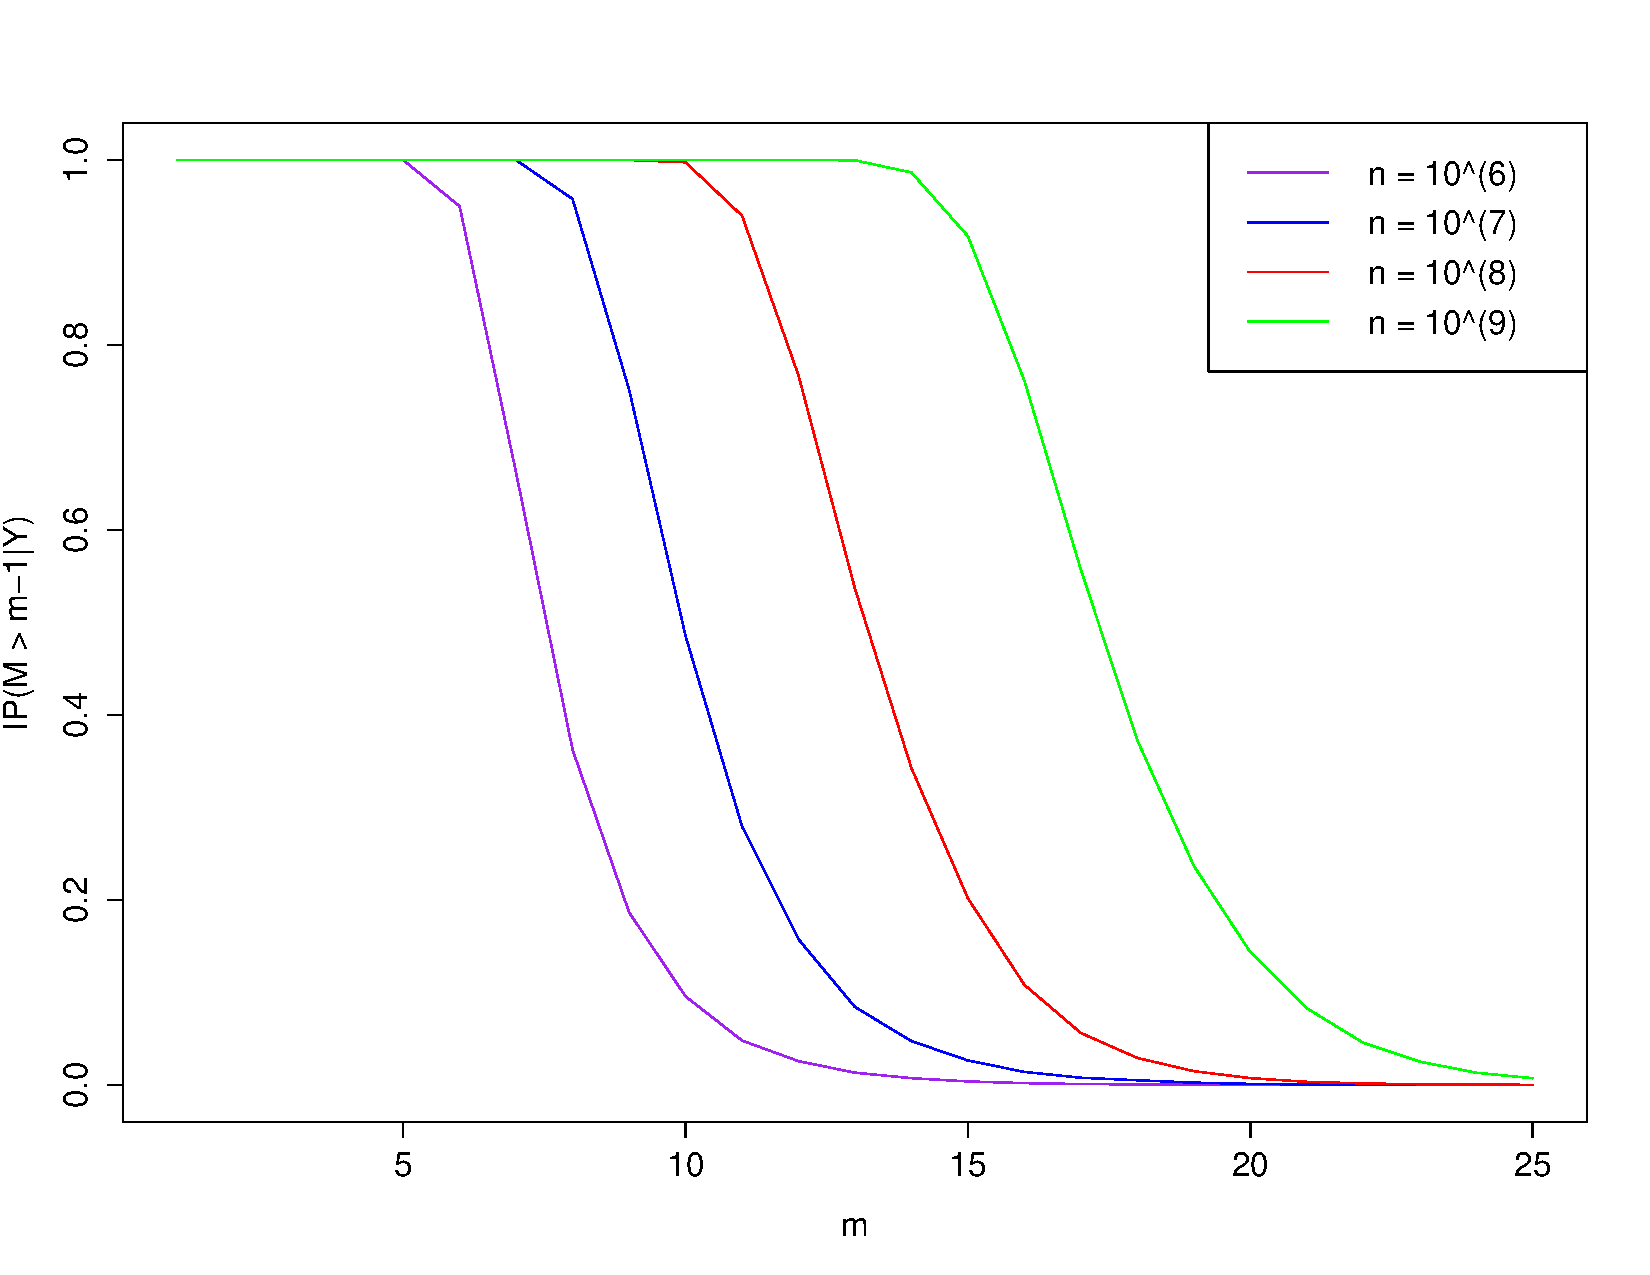
\includegraphics[width=1\linewidth]{M.pdf}
%\caption{Survival function of $M$ for different values of $n$}\label{M}
%\end{figure}
%\end{column}
%\end{columns} % End of the subdivision
\begin{itemize}
\item Hence, given $M$, the posterior is
\begin{align*}
\forall j > m, &\quad \boldsymbol{\theta}_{j} \vert M = m, Y \sim \delta_{0},\\
\forall j \leq m, &\quad \boldsymbol{\theta}_{j} \vert M = m, Y \sim \mathcal{N}\left(\frac{Y_{j} \cdot n \cdot \lambda_{j}}{1 + n \cdot \lambda_{j}^{2}}, \frac{1}{1 + n \cdot \lambda_{j}^{2}} \right).
\end{align*}
\end{itemize}
\underline{Remark:} the family of hierarchical priors with deterministic threshold $M$ is called family of sieve priors.

\begin{figure}
\centering
 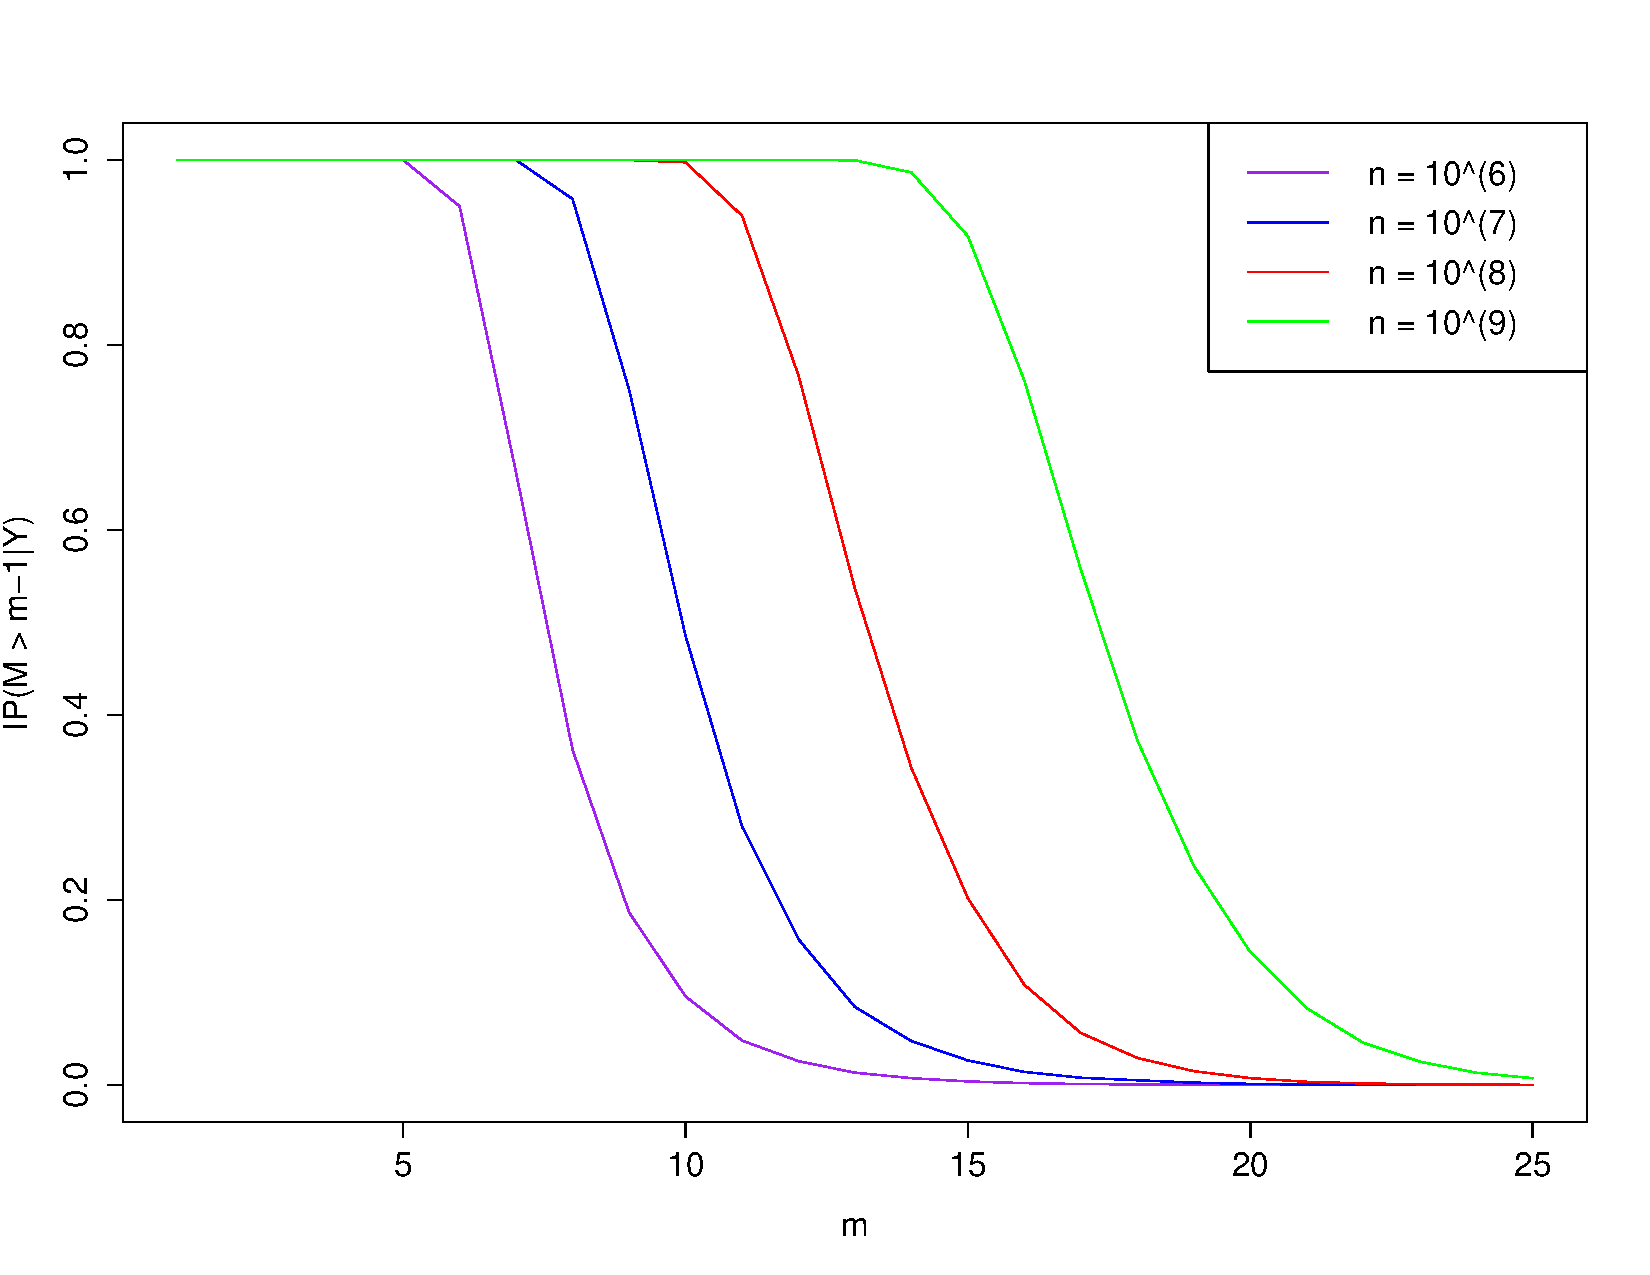
\includegraphics[width=0.4\linewidth]{M.pdf}
\caption{Survival function of $M$ for different values of $n$}\label{M}
\end{figure}

\end{block}

\end{column} % End of the first column

\begin{column}{.02\textwidth}\end{column} % Empty spacer column

\begin{column}{.30\textwidth} % The first column

%----------------------------------------------------------------------------------------
%	EXISTING RESULTS
%----------------------------------------------------------------------------------------

\begin{block}{\rule{0pt}{2.5ex} Existing results}
In \citet{JJASRS}, under a \textcolor{red!90!black}{pragmatic Bayesian} point of view; that is, the existence of a true parameter $\theta^{\circ}$ is accepted; it is shown that, by choosing $\mathbb{P}_{M}$ suitably:
\begin{itemize}
	\item the estimator $\widehat{\theta}^{\left(1\right)}$ \textcolor{red!90!black}{converges with,}
	\begin{itemize}
		\item \textcolor{red!90!black}{oracle optimal rate} for the quadratic risk which means, $\forall \theta^{\circ} \in \Theta^{\circ}, \exists C^{\circ} \in \left[ 1, \infty \right[ : \forall n \in \mathbb{N}, \exists \Phi_{n}^{\circ} \in \mathbb{R}:$
		\begin{alignat*}{2}
&\inf\limits_{m \in \mathbb{N}} \, && \mathbb{E}_{\theta^{\circ}}^{n}\left[\left\Vert \tilde{\theta}^{m} - \theta^{\circ} \right\Vert^{2}\right] \geq \Phi_{n}^{\circ},\\
& && \mathbb{E}_{\theta^{\circ}}^{n}\left[\left\Vert \widehat{\theta}^{\left(1\right)} - \theta^{\circ} \right\Vert^{2}\right] \leq C^{\circ} \Phi_{n}^{\circ};
		\end{alignat*}
		\item \textcolor{red!90!black}{minimax optimal rate} for the maximal risk over $\Theta^{\circ}$, that is to say, $\exists C^{\star} \in \left[ 1, \infty \right[ : \forall n \in \mathbb{N}, \exists \Phi_{n}^{\star} \in \mathbb{R}:$
\begin{alignat*}{2}
& \inf\limits_{\tilde{\theta}} &&\sup\limits_{\theta^{\circ} \in \Theta^{\circ}} \mathbb{E}_{\theta^{\circ}}^{n}\left[\left\Vert \tilde{\theta} - \theta^{\circ} \right\Vert^{2}\right] \geq \Phi_{n}^{\star},\\
& && \sup\limits_{\theta^{\circ} \in \Theta^{\circ}} \mathbb{E}_{\theta^{\circ}}^{n}\left[\left\Vert \widehat{\theta}^{\left(1\right)} - \theta^{\circ} \right\Vert^{2}\right] \leq C^{\star} \Phi_{n}^{\star},
\end{alignat*}
where $\inf\limits_{\tilde{\theta}}$ is taken over all possible estimators of $\theta^{\circ}$;
	\end{itemize}
	\item the posterior distribution \textcolor{red!90!black}{concentrates with,}
	\begin{itemize}
		\item \textcolor{red!90!black}{oracle optimal rate} for the quadratic loss which means, $\forall \theta^{\circ} \in \Theta^{\circ}, \exists K^{\circ} \in \left[ 1, \infty \right[ :$
\[\lim\limits_{n \rightarrow \infty} \mathbb{E}_{\theta^{\circ}}^{n}\left[\mathbb{P}_{\boldsymbol{\theta}^{1}\vert Y^{1}}^{n}\left(\left\Vert \boldsymbol{\theta} - \theta^{\circ} \right\Vert^{2} \leq K^{\circ} \Phi_{n}^{\circ}\right)\right] = 1;\]
		\item \textcolor{red!90!black}{minimax optimal rate} $\Theta^{\circ}$, that is to say, for any unbounded sequence $K_{n} \in \mathbb{R}^{\mathbb{N}} :$
\[\lim\limits_{n \rightarrow \infty} \sup\limits_{\theta^{\circ} \in \Theta^{\circ}}  \mathbb{E}_{\theta^{\circ}}^{n}\left[\mathbb{P}_{\boldsymbol{\theta}^{1}\vert Y^{1}}^{n}\left(\left\Vert \boldsymbol{\theta} - \theta^{\circ} \right\Vert^{2} \leq K_{n} \Phi_{n}^{\star}\right)\right] = 1.\]
	\end{itemize}

%	\item the posterior distribution \textcolor{red!90!black}{concentrates with,}
%	\begin{itemize}
%		\item \textcolor{red!90!black}{oracle optimal rate} for the quadratic loss over the class of priors with deterministic threshold which means, $\forall \theta^{\circ} \in \Theta^{\circ}, \exists \Phi_{n}^{\circ} \in \mathbb{R}^{\mathbb{N}}, K^{\circ} \in \left[ 1, \infty \right[ :$
%		\begin{alignat*}{3}
%& \inf\limits_{P_{\boldsymbol{\theta}}} \,&& \lim\limits_{n \rightarrow \infty}\mathbb{E}_{\theta^{\circ}}&&\left[P_{\boldsymbol{\theta}\vert Y}\left(\left\Vert \boldsymbol{\theta} - \theta^{\circ} \right\Vert^{2} \geq \Phi_{n}^{\circ}\right)\right] = 1,\\
%& &&\lim\limits_{n \rightarrow \infty} \mathbb{E}_{\theta^{\circ}}&&\left[\mathbb{P}_{\boldsymbol{\theta}\vert Y}\left(\left\Vert \boldsymbol{\theta} - \theta^{\circ} \right\Vert^{2} \leq K^{\circ} \Phi_{n}^{\circ}\right)\right] = 1,
%\end{alignat*}
%where $\inf\limits_{P_{\boldsymbol{\theta}}}$ is taken over the family of sieve prior distributions for $\boldsymbol{\theta}$;
%		\item \textcolor{red!90!black}{minimax optimal rate} for the maximal risk over $\Theta^{\circ}$, defined as above, that is to say, $\exists \Phi_{n}^{\star} \in \mathbb{R}^{\mathbb{N}}, K^{\star} \in \left[ 1, \infty \right[ :$
%		\begin{alignat*}{2}
%& \inf\limits_{P_{\boldsymbol{\theta}}} &&\sup\limits_{\theta^{\circ} \in \Theta^{\circ}} \lim\limits_{n \rightarrow \infty} \mathbb{E}_{\theta^{\circ}}\left[P_{\boldsymbol{\theta}\vert Y}\left(\left\Vert \boldsymbol{\theta} - \theta^{\circ} \right\Vert^{2} \geq \Phi_{n}^{\star}\right)\right] = 1,\\
%& && \sup\limits_{\theta^{\circ} \in \Theta^{\circ}} \lim\limits_{n \rightarrow \infty} \mathbb{E}_{\theta^{\circ}}\left[\mathbb{P}_{\boldsymbol{\theta}\vert Y}\left(\left\Vert \boldsymbol{\theta} - \theta^{\circ} \right\Vert^{2} \leq K^{\star} \Phi_{n}^{\star}\right)\right] = 1,
%\end{alignat*}
%where $\inf\limits_{P_{\boldsymbol{\theta}}}$ is taken over all possible sieve priors for $\boldsymbol{\theta}$;
%	\end{itemize}
\end{itemize}
\end{block}

%----------------------------------------------------------------------------------------
%	ITERATED POSTERIOR DISTRIBUTION
%----------------------------------------------------------------------------------------

%\begin{block}{\centering Iterated posterior distributions and self informative limits}
%
%In the spirit of \citet{OBJJ}, we generate a posterior family by introducing an \textcolor{red!90!black}{iteration parameter $\eta$} such that :
%\begin{itemize}
%\item for $\eta = 1$, the situation is the same as before, the prior distribution is $\mathbb{P}_{\boldsymbol{\theta}}$ and the posterior distribution is $\mathbb{P}_{\boldsymbol{\theta}\vert Y}$,
%\item for $\eta = 2$, we take the posterior for $\eta = 1$ as prior, hence, the prior distribution is $\mathbb{P}_{\boldsymbol{\theta} \vert Y}$ and we compute the posterior distribution with the same observations $Y$, which we note $\mathbb{P}_{\boldsymbol{\theta}\vert Y^{\left(2\right)}}$,
%\item $\hdots$
%\item for any value of $\eta > 1,$ our prior is \textcolor{red!90!black}{$\mathbb{P}_{\boldsymbol{\theta} \vert Y^{\left(\eta - 1\right)}}$} and we compute the posterior with the same observation $Y$ which is \textcolor{red!90!black}{$\mathbb{P}_{\boldsymbol{\theta} \vert Y^{\left(\eta\right)}}$}.
%\end{itemize}
%
%This iteration procedure corresponds to giving more and more weight to the observations and make the prior knowledge vanish.
%We are interested into the behavior of all the elements of the family $\left(\mathbb{P}_{\boldsymbol{\theta}\vert Y^{\left(\eta\right)}}\right)_{\eta \in \mathbb{N}^{\star}}$ as well as the distribution obtained when we let $\eta$ tend to infinite, called self-informative limit.
%
%\medskip
%
%Within this framework we define the family of estimators given by the posterior means for each value of $\eta$ :
%\[\textcolor{red!90!black}{\widehat{\theta}^{\left(\eta\right)} := \mathbb{E}_{\boldsymbol{\theta}\vert Y^{\left(\eta\right)}}\left[\boldsymbol{\theta}\right]}.\]
%\end{block}

%----------------------------------------------------------------------------------------
%	FAMILY OF POSTERIOR DISTRIBUTIONS
%----------------------------------------------------------------------------------------

\begin{block}{\rule{0pt}{2.5ex} Iterated posterior distributions}
Note that in the framework of our hierarchical prior, we have:
\textcolor{red!90!black}{
\begin{alignat*}{2}
&\mathbb{P}_{\boldsymbol{\theta}^{\eta}\vert Y^{\eta}}^{n} &&= \sum\limits_{m \in \mathbb{N}} \mathbb{P}_{\boldsymbol{\theta}^{\eta} \vert M^{\eta} = m, Y^{\eta}}^{n} \cdot \mathbb{P}^{n}_{M^{\eta} = m \vert Y^{\eta}},\\
&\widehat{\theta}^{\left(\eta\right)} &&= \left(\mathbb{E}_{\boldsymbol{\theta}^{\eta}\vert M^{\eta} \geq j, Y^{\eta}}^{n}\left[\boldsymbol{\theta}_{j}\right] \cdot \mathbb{P}_{M^{\eta} \vert Y^{\eta}}^{n}\left(M^{\eta} \geq j\right)\right)_{j \in \mathbb{N}}.
\end{alignat*}}

Hence, we first compute $\boldsymbol{\theta}^{\eta}_{j} \vert M^{\eta}, Y^{\eta}$:
\textcolor{red!90!black}{\begin{alignat*}{4}
& \forall j \in \mathbb{N}, && \quad \boldsymbol{\theta}^{\eta}_{j} \vert M^{\eta} \geq j, Y^{\eta} &&\sim &&\mathcal{N}\left(\frac{\eta \cdot Y_{j} \cdot n \cdot \lambda_{j}}{1 + \eta \cdot n \cdot \lambda_{j}^{2}}, \frac{1}{1 + n \cdot \eta \cdot \lambda_{j}^{2}} \right),\\
&  && \quad \boldsymbol{\theta}^{\eta}_{j} \vert M^{\eta} < j, Y^{\eta} &&\sim &&\delta_{0};
\end{alignat*}}

and then fix the distribution of $M^{1}$: $\forall m \in \llbracket 1, G_{n} \rrbracket, $
%\[\mathbb{P}_{M}(M = m) := \frac{\exp\left(-3 \cdot \eta \cdot \frac{m}{2} \right) \cdot \prod\limits_{j = 1}^{m} \left(1 + n \cdot \eta \cdot \lambda_{j}^{2}\right)^{2}}{\sum\limits_{k =1}^{G_{n}} \exp\left(-3 \cdot \eta \cdot \frac{k}{2} \right) \cdot \prod\limits_{j = 1}^{k} \left(1 + n \cdot \eta \cdot \lambda_{j}^{2}\right)^{2}}.\]
\[\mathbb{P}_{M^{1}}(M = m) \propto \exp\left(-3 \cdot \eta \cdot \frac{m}{2} \right) \cdot \prod\limits_{j = 1}^{m} \left(1 + n \cdot \eta \cdot \lambda_{j}^{2}\right)^{2}.\]
%\begin{columns} % Subdivide the first main column
%\begin{column}{.5\textwidth} % The first subdivided column within the first main column
Which gives the family of posterior distributions:
\textcolor{red!90!black}{\[\mathbb{P}_{M^{\eta} \vert Y^{\eta}}^{n}(m) \propto \exp\!\!\left[- \frac{\eta}{2} \left( 3 m - \sum\limits_{j = 1}^{m} \frac{\eta\left(Y_{j} \cdot n \cdot \lambda_{j}^{2}\right)^{2}}{1 + \eta \cdot n \cdot \lambda_{j}^{2}} \right)\right].\]}
%\end{column}
%\begin{column}{.5\textwidth} % The first subdivided column within the first main column
%\begin{figure}[H]
%\caption{Survival function of $M$ for different values of $\eta$}
%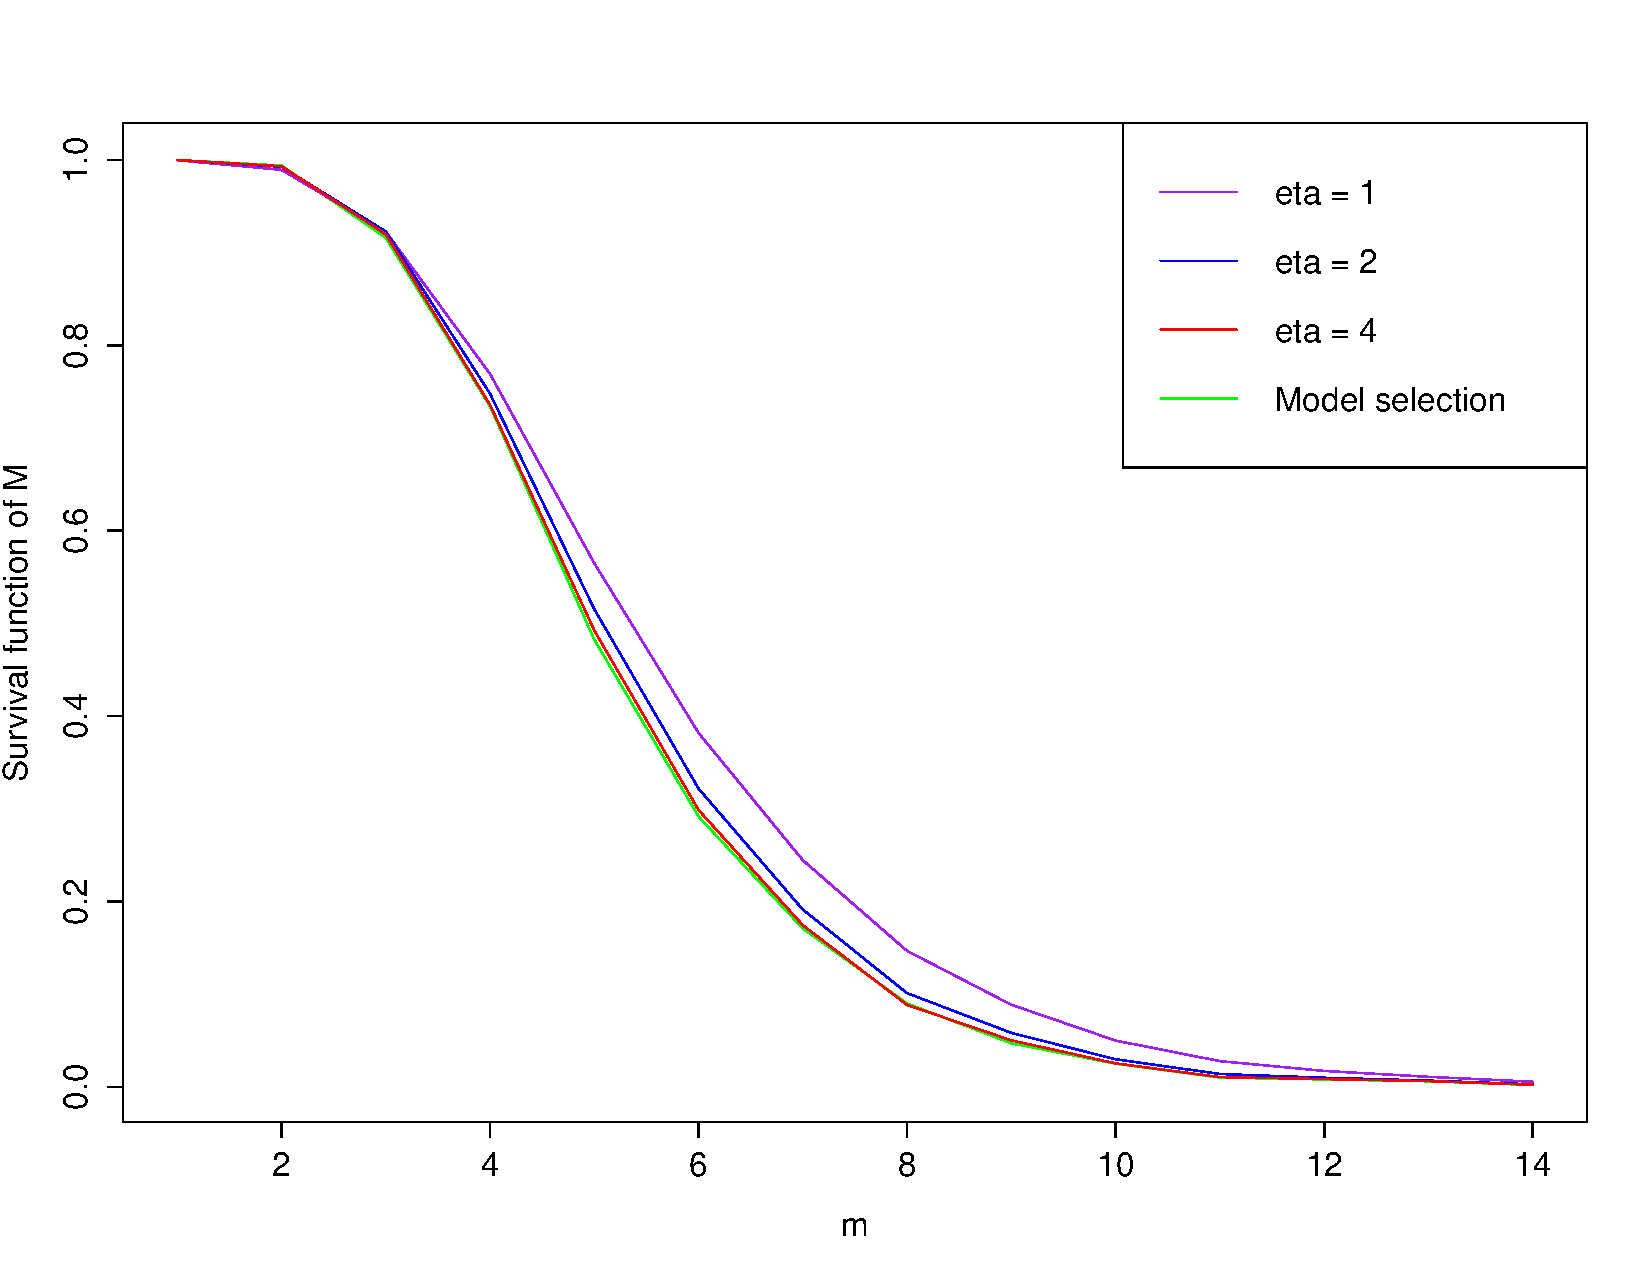
\includegraphics[width = 13.5cm]{iteration.pdf}\hfill
%\end{figure}
%\end{column}
%\end{columns}
\end{block}

%----------------------------------------------------------------------------------------
%	SELF INFORMATIVE LIMIT
%----------------------------------------------------------------------------------------

\begin{block}{\rule{0pt}{2.5ex} Self informative limit and model selection}
Consider the limit of the family of posteriors as $\eta$ tends to infinite:
\[\lim_{\eta \rightarrow \infty} \mathbb{P}_{\boldsymbol{\theta}^{\eta} \vert M^{\eta} = m, Y^{\eta}}^{n} = \delta_{\tilde{\theta}^{m}},\]
where $\tilde{\theta}^{m}$ is the projection estimator on the first $m$ dimensions.

The distribution of $M$ tends to a point mass:
\[\lim_{\eta \rightarrow \infty} \mathbb{P}_{M^{\eta}\vert Y^{\eta}}^{n} = \delta_{\widehat{m}},\]
where $\widehat{m}$ is the choice given by the frequentist model selection presented earlier.

\medskip

The \textcolor{red}{self-informative limit} is equal to the model selection estimator, $\widehat{\theta}$, presented above.

\begin{figure}[H]
\caption{Survival function of $M$ for different values of $\eta$}
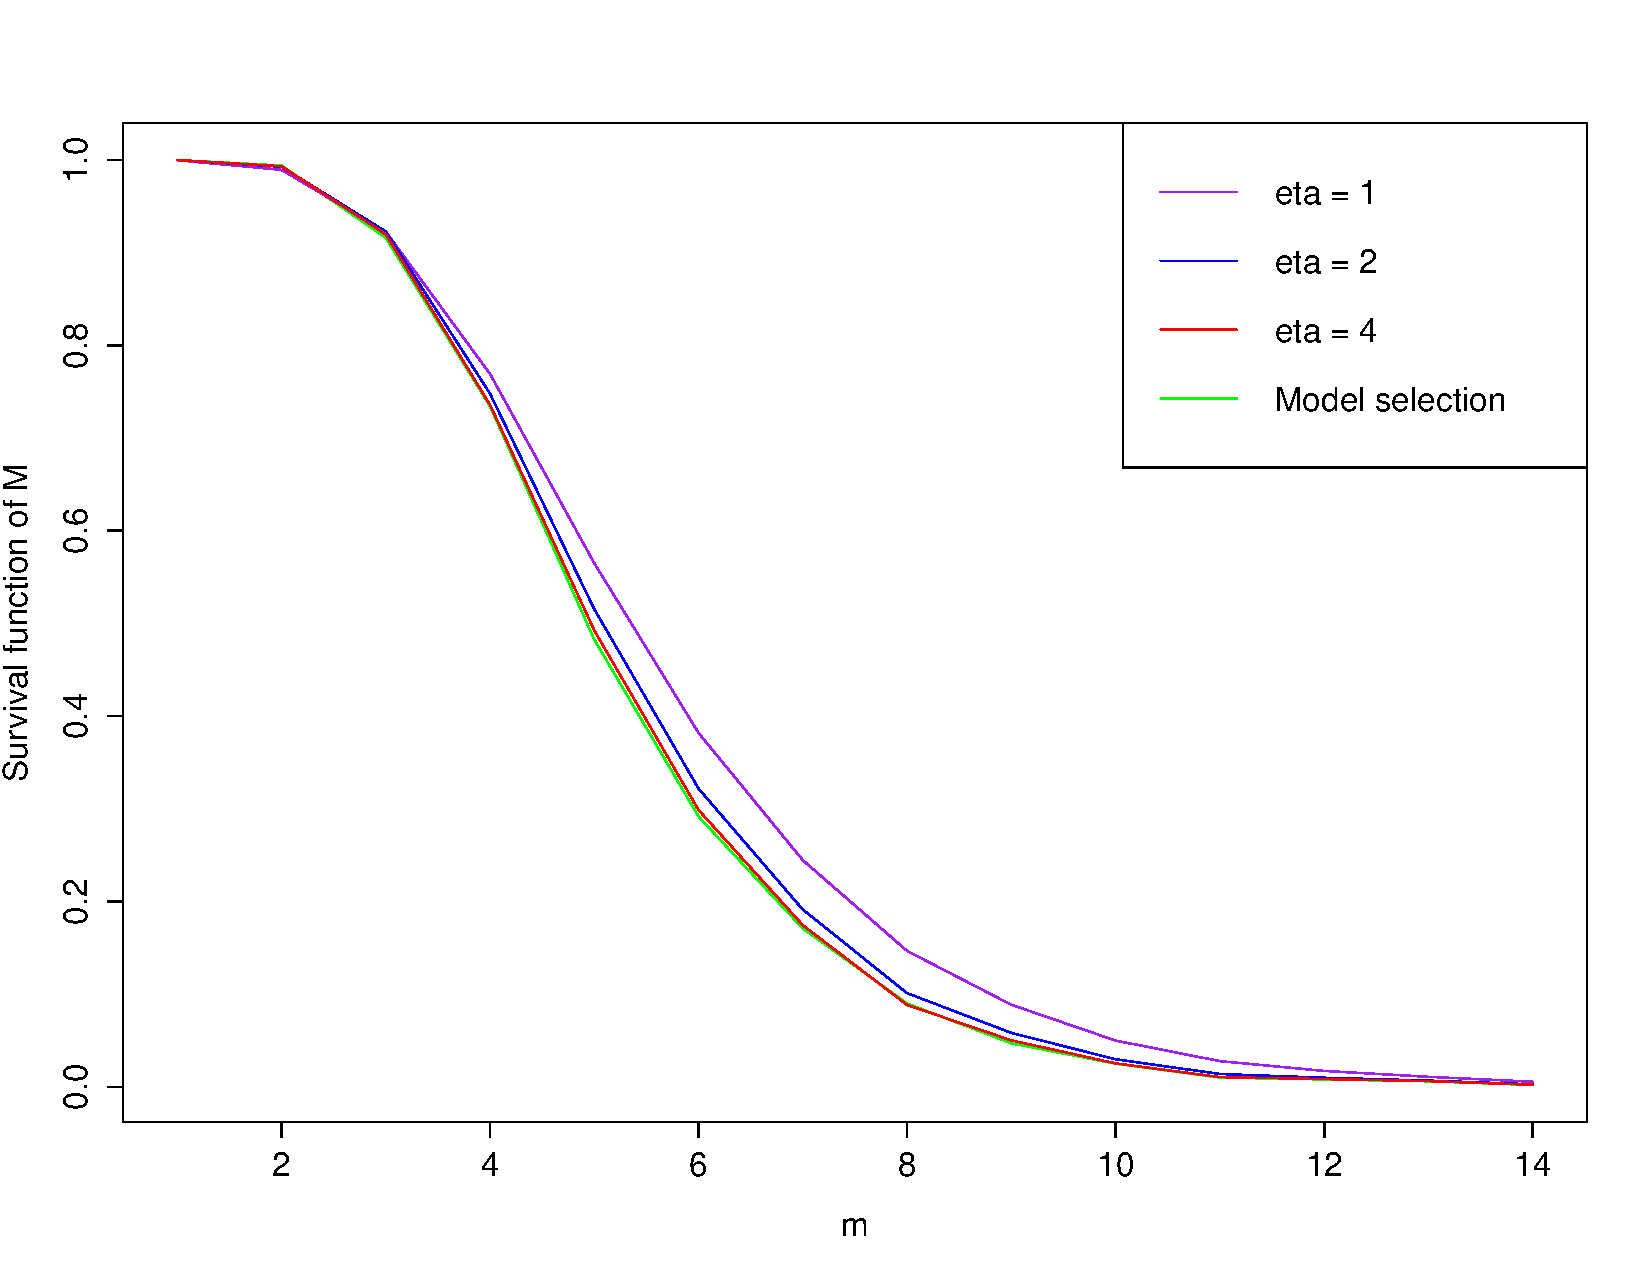
\includegraphics[width=0.5\linewidth]{iteration.pdf}\hfill
\end{figure}

\end{block}

%----------------------------------------------------------------------------------------
%	DEFINITIONS
%----------------------------------------------------------------------------------------

\begin{block}{\rule{0pt}{2.5ex} Notations}
Define the following quantities:
\[\textgoth{b}_{m} := \sum\limits_{j = m + 1}^{\infty} \left(\theta^{\circ}\right)^{2}, \quad \Lambda_{j} := \lambda_{j}^{-2}, \quad m \cdot \overline{\Lambda}_{m} := \sum\limits_{j = 1}^{m} \Lambda_{j},\]
\begin{alignat*}{3}
&m_{n}^{\circ} &&:= \argmin\limits_{m \in \llbracket 1, G_{n} \rrbracket} \left[\textgoth{b}_{m} \vee n^{-1} m \overline{\Lambda}_{m}\right], && \quad \Phi_{n}^{\circ} := \left[\textgoth{b}_{m_{n}^{\circ}}\vee n^{-1} m_{n}^{\circ} \overline{\Lambda}_{m_{n}^{\circ}}\right],\\
&m_{n}^{\star} &&:= \argmin\limits_{m \in \llbracket 1, G_{n} \rrbracket} \left[\textgoth{a}_{m} \vee n^{-1} m \overline{\Lambda}_{m}\right], && \quad \Phi_{n}^{\star} := \left[\textgoth{a}_{m_{n}^{\star}} \vee n^{-1} m_{n}^{\star} \overline{\Lambda}_{m_{n}^{\star}}\right].
\end{alignat*}

It is important to note that:
\begin{itemize}
\item $\Phi_{n}^{\star}$ is the minimax optimal rate over $\Theta^{\circ}$,
\item $\Phi_{n}^{\circ}$ is the oracle optimal rate over the projection estimators.
\end{itemize}
\end{block}

\end{column} % End of the first column

\begin{column}{.02\textwidth}\end{column} % Empty spacer column
 
\begin{column}{.30\textwidth} % The second column

%----------------------------------------------------------------------------------------
%	PRAGMATIC BAYESIAN AND MINIMAX THEORY
%----------------------------------------------------------------------------------------

%\begin{block}{Pragmatic Bayesian point of view}
%
%To quantify the quality of the posterior distribution assume the existence of a true parameter $\theta^{\circ}$ which belongs to some parameter space $\Theta^{\circ}$, we then define
%\begin{itemize}
%\item an exact concentration rate, a sequence $\Phi_{n}^{\circ}$ such that there exist $K^{\circ} \geq 1$ for which, with all $\theta^{\circ}$
%\[\lim\limits_{n \rightarrow \infty} \mathbb{E}_{\theta}^{\circ} \left[\mathbb{P}_{\boldsymbol{\theta}, M \vert Y^{\eta}}\left(\left(K^{\circ}\right)^{-1} \Phi_{n}^{\circ} \leq \left\Vert \boldsymbol{\theta} - \theta^{\circ} \right\Vert^{2} \leq K^{\circ} \Phi_{n}^{\circ}\right)\right] = 1,\]
%\item an exact uniform concentration rate, a sequence $\Phi_{n}^{\star}$ such that there exist $K^{\circ} \geq 1$ for which
%\[\lim\limits_{n \rightarrow \infty} \inf\limits_{\theta^{\circ} \in \Theta^{\circ}}\mathbb{E}_{\theta}^{\circ} \left[\mathbb{P}_{\boldsymbol{\theta}, M \vert Y^{\eta}}\left(\left(K^{\star}\right)^{-1} \Phi_{n}^{\star} \leq \left\Vert \boldsymbol{\theta} - \theta^{\circ} \right\Vert^{2} \leq K^{\star} \Phi_{n}^{\star}\right)\right] = 1.\]
%\end{itemize}
%
%\end{block}

%----------------------------------------------------------------------------------------
%	ASSUMPTIONS
%----------------------------------------------------------------------------------------

\begin{block}{\rule{0pt}{2.5ex} Set of assumptions}
Define the following assumptions:
\begin{alignat*}{2}
&\left(\mathbb{H}_{\lambda}\right) &&: \exists a \in \mathbb{R}_{+}, c \geq 1 : \quad \forall j \in \mathbb{N}, \quad \left(\frac{1}{c} j^{-a} \leq \lambda_{j} \leq c j^{-a}\right)\\
&\left(\mathbb{H}_{1}\right) &&: 0 <\inf\limits_{n \in \mathbb{N}} \left\{\frac{\left[\textgoth{b}_{m_{n}^{\circ}}\wedge n^{-1} m_{n}^{\circ} \overline{\Lambda}_{m_{n}^{\circ}}\right]}{\left[\textgoth{b}_{m_{n}^{\circ}}\vee n^{-1} m_{n}^{\circ} \overline{\Lambda}_{m_{n}^{\circ}}\right]}\right\} \leq 1\\
&\left(\mathbb{H}_{2}\right) &&: 0 <\inf\limits_{n \in \mathbb{N}} \left\{\frac{\left[\textgoth{a}_{m_{n}^{\star}}\wedge n^{-1} m_{n}^{\star} \overline{\Lambda}_{m_{n}^{\star}}\right]}{\left[\textgoth{a}_{m_{n}^{\star}}\vee n^{-1} m_{n}^{\star} \overline{\Lambda}_{m_{n}^{\star}}\right]}\right\} \leq 1\\
\end{alignat*}
Note that under $\left(\mathbb{H}_{\lambda}\right)$, there exist a constant $L$ such that,
\[\forall m \in \mathbb{N}, \quad \Lambda_{m} \leq L \overline{\Lambda}_{m}.\]
\end{block}

%----------------------------------------------------------------------------------------
%	CONCENTRATION FOR M
%----------------------------------------------------------------------------------------
\setbeamercolor{block title}{fg=white,bg=red!90!black}
\begin{block}{\rule{0pt}{2.5ex} Concentration results for the threshold parameter $M$}
For any $\eta$ in $\overline{\mathbb{N}},$ we have the following results:

\medskip

\begin{enumerate}
\item Under assumptions $\left(\mathbb{H}_{1}\right)$ and $\left(\mathbb{H}_{\lambda}\right)$, define
\begin{alignat*}{2}
&G_{n}^{-} &&:= \min\left\{m \in \llbracket 1, m_{n}^{\circ} \rrbracket : \textgoth{b}_{m} \leq 9 L \Phi_{n}^{\circ}\right\},\\
&G_{n}^{+} &&:= \max \left\{m \in \llbracket m_{n}^{\circ}, G_{n} \rrbracket : \left( m - m_{n}^{\circ} \right) n^{-1} \leq 3 \Lambda_{m_{n}^{\circ}}^{-1} \Phi_{n}^{\circ}\right\},
\end{alignat*}
and we then have the following concentration for $M$,
\begin{alignat*}{4}
&\mathbb{P}_{M^{\eta} \vert Y^{\eta}}^{n}&&\left[M > G_{n}^{+}\right] &&\leq&& \exp\left[- \frac{5 m_{n}^{\circ}}{9 L} + \log \left(G_{n}\right)\right],\\
&\mathbb{P}_{M^{\eta} \vert Y^{\eta}}^{n}&&\left[M < G_{n}^{-}\right] &&\leq&& \exp\left[- \frac{7 m_{n}^{\circ}}{9} + \log \left(G_{n}\right)\right],
\end{alignat*}
\textcolor{red!90!black}{this means that $M^{\eta}$ tends to select an oracle optimal threshold};
\item whereas under $\left(\mathbb{H}_{2}\right)$ and $\left(\mathbb{H}_{\lambda}\right)$, we define
\begin{alignat*}{2}
&G_{n}^{\star-} &&:= \min\left\{m \in \llbracket 1, m_{n}^{\star} \rrbracket : \quad \textgoth{b}_{m} \leq 9 \left(1 \vee L^{\circ}\right) L \Phi_{n}^{\star}\right\},\\
&G_{n}^{\star+} &&:= \max \left\{m \in \llbracket m_{n}^{\star}, G_{n} \rrbracket : \left( m - m_{n}^{\star} \right) n^{-1} \leq 3 \Lambda_{m_{n}^{\star}}^{-1} \left(1 \vee L^{\circ}\right) \Phi_{n}^{\star}\right\},
\end{alignat*}
and the following concentration stands,
\begin{alignat*}{4}
&\mathbb{P}_{M^{\eta} \vert Y^{\eta}}^{n}&&\left[M > G_{n}^{\star+}\right] &&\leq &&\exp\left[- \frac{5 \left(1 \vee L^{\circ}\right) m_{n}^{\star}}{9 L} + \log \left(G_{n}\right)\right],\\
&\mathbb{P}_{M^{\eta} \vert Y^{\eta}}^{n}&&\left[M < G_{n}^{\star-}\right] &&\leq &&\exp\left[- \frac{7 \left(1 \vee L^{\circ}\right) m_{n}^{\star}}{9} + \log \left(G_{n}\right)\right],
\end{alignat*}
\textcolor{red!90!black}{which means that $M^{\eta}$ tends to select a minimax optimal threshold}.
\end{enumerate}
\end{block}


%----------------------------------------------------------------------------------------
%	CONCENTRATION FOR THETA
%----------------------------------------------------------------------------------------
\setbeamercolor{block title}{fg=white,bg=red!90!black}
\begin{block}{\rule{0pt}{2.5ex} Concentration results for $\boldsymbol{\theta}$}
For any $\eta$ in $\mathbb{N},$ we have the following results:

\medskip

\begin{enumerate}
\item under assumptions $\left(\mathbb{H}_{1}\right)$ and $\left(\mathbb{H}_{\lambda}\right)$, for all $\theta^{\circ}$ in $\Theta^{\circ}$, there exist $K^{\circ} \geq 1$ and $C^{\circ} > 1$ such that we have
\begin{alignat*}{3}
& \lim\limits_{n \rightarrow \infty}&& \inf\limits_{\mathbb{Q}_{\boldsymbol{\theta}}}\,&& \mathbb{E}_{\theta^{\circ}}^{n}\left[\mathbb{Q}_{\boldsymbol{\theta} \vert Y}^{n}\left(\left\Vert \boldsymbol{\theta} - \theta^{\circ} \right\Vert^{2} \geq \Phi_{n}^{\circ}\right)\right] = 1,\\
&\lim\limits_{n \rightarrow \infty} &&\mathbb{E}_{\theta^{\circ}}^{n}&&\left[\mathbb{P}_{\boldsymbol{\theta}^{\eta}, M^{\eta} \vert Y^{\eta}}^{n}\left(\left(K^{\circ}\right)^{-1} \Phi_{n}^{\circ} \leq \Vert \boldsymbol{\theta} - \theta^{\circ} \Vert^{2} \leq K^{\circ} \Phi_{n}^{\circ} \right)\right] = 1,\\
& &&\mathbb{E}_{\theta^{\circ}}^{n}&&\left[\Vert \widehat{\theta}^{\left(\eta\right)} - \theta^{\circ} \Vert^{2}\right] \leq C^{\circ} \Phi_{n}^{\circ},
\end{alignat*}
where $\inf_{\mathbb{Q}_{\boldsymbol{\theta}}}$ is taken over all possible sieve priors; \textcolor{red!90!black}{establishing oracle optimal concentration and convergence of the posterior and Bayes estimate, respectively};
\item whereas under $\left(\mathbb{H}_{2}\right)$ and $\left(\mathbb{H}_{\lambda}\right)$, for a finite constant $C^{\star} \geq 1$ and any unbounded sequence $K_{n}$, we have
\begin{alignat*}{4}
& \lim\limits_{n \rightarrow \infty} && \inf\limits_{\mathbb{Q}_{\boldsymbol{\theta}}}\sup\limits_{\theta^{\circ} \in \Theta^{\circ}}\,&& \mathbb{E}_{\theta^{\circ}}^{n}&&\left[\mathbb{Q}_{\boldsymbol{\theta} \vert Y}^{n}\left(\left\Vert \boldsymbol{\theta} - \theta^{\circ} \right\Vert^{2} \geq \Phi_{n}^{\star}\right)\right] = 1,\\
& \lim\limits_{n \rightarrow \infty} && \sup\limits_{\theta^{\circ} \in \Theta^{\circ}}&& \mathbb{E}_{\theta^{\circ}}^{n}&&\left[\mathbb{P}_{\boldsymbol{\theta}^{\eta}, M^{\eta} \vert Y^{\eta}}^{n}\left(\Vert \boldsymbol{\theta} - \theta^{\circ} \Vert^{2} \leq K_{n} \Phi_{n}^{\star} \right)\right] = 1,\\
& &&\sup\limits_{\theta^{\circ}\in \Theta^{\circ}}&&\mathbb{E}_{\theta^{\circ}}^{n}&&\left[\Vert \widehat{\theta}^{\left(\eta\right)} - \theta^{\circ} \Vert^{2}\right] \leq C^{\star} \Phi_{n}^{\star},
\end{alignat*}
where $\inf_{\mathbb{Q}_{\boldsymbol{\theta}}}$ is taken over all possible sieve priors; \textcolor{red!90!black}{establishing minimax optimal concentration and convergence of the posterior and Bayes estimate, respectively}.
\end{enumerate}

\textcolor{red!90!black}{Note that in the case of $\eta \rightarrow \infty$, those results are still true and that the concentration corresponds to the convergence in probability} as
\[\lim\limits_{\eta \rightarrow \infty}\mathbb{E}_{\theta^{\circ}}^{n}\left[\mathbb{P}_{\boldsymbol{\theta}^{\eta}, M^{\eta} \vert Y^{\eta}}^{n}\left(\Vert \boldsymbol{\theta} - \theta^{\circ} \Vert^{2} \leq K_{n} \Phi_{n} \right)\right] = \mathbb{P}_{\theta^{\circ}}^{n}\left[\Vert \widehat{\theta} - \theta^{\circ} \Vert^{2} \leq K_{n} \Phi_{n}\right].\]

\begin{figure}
\centering
  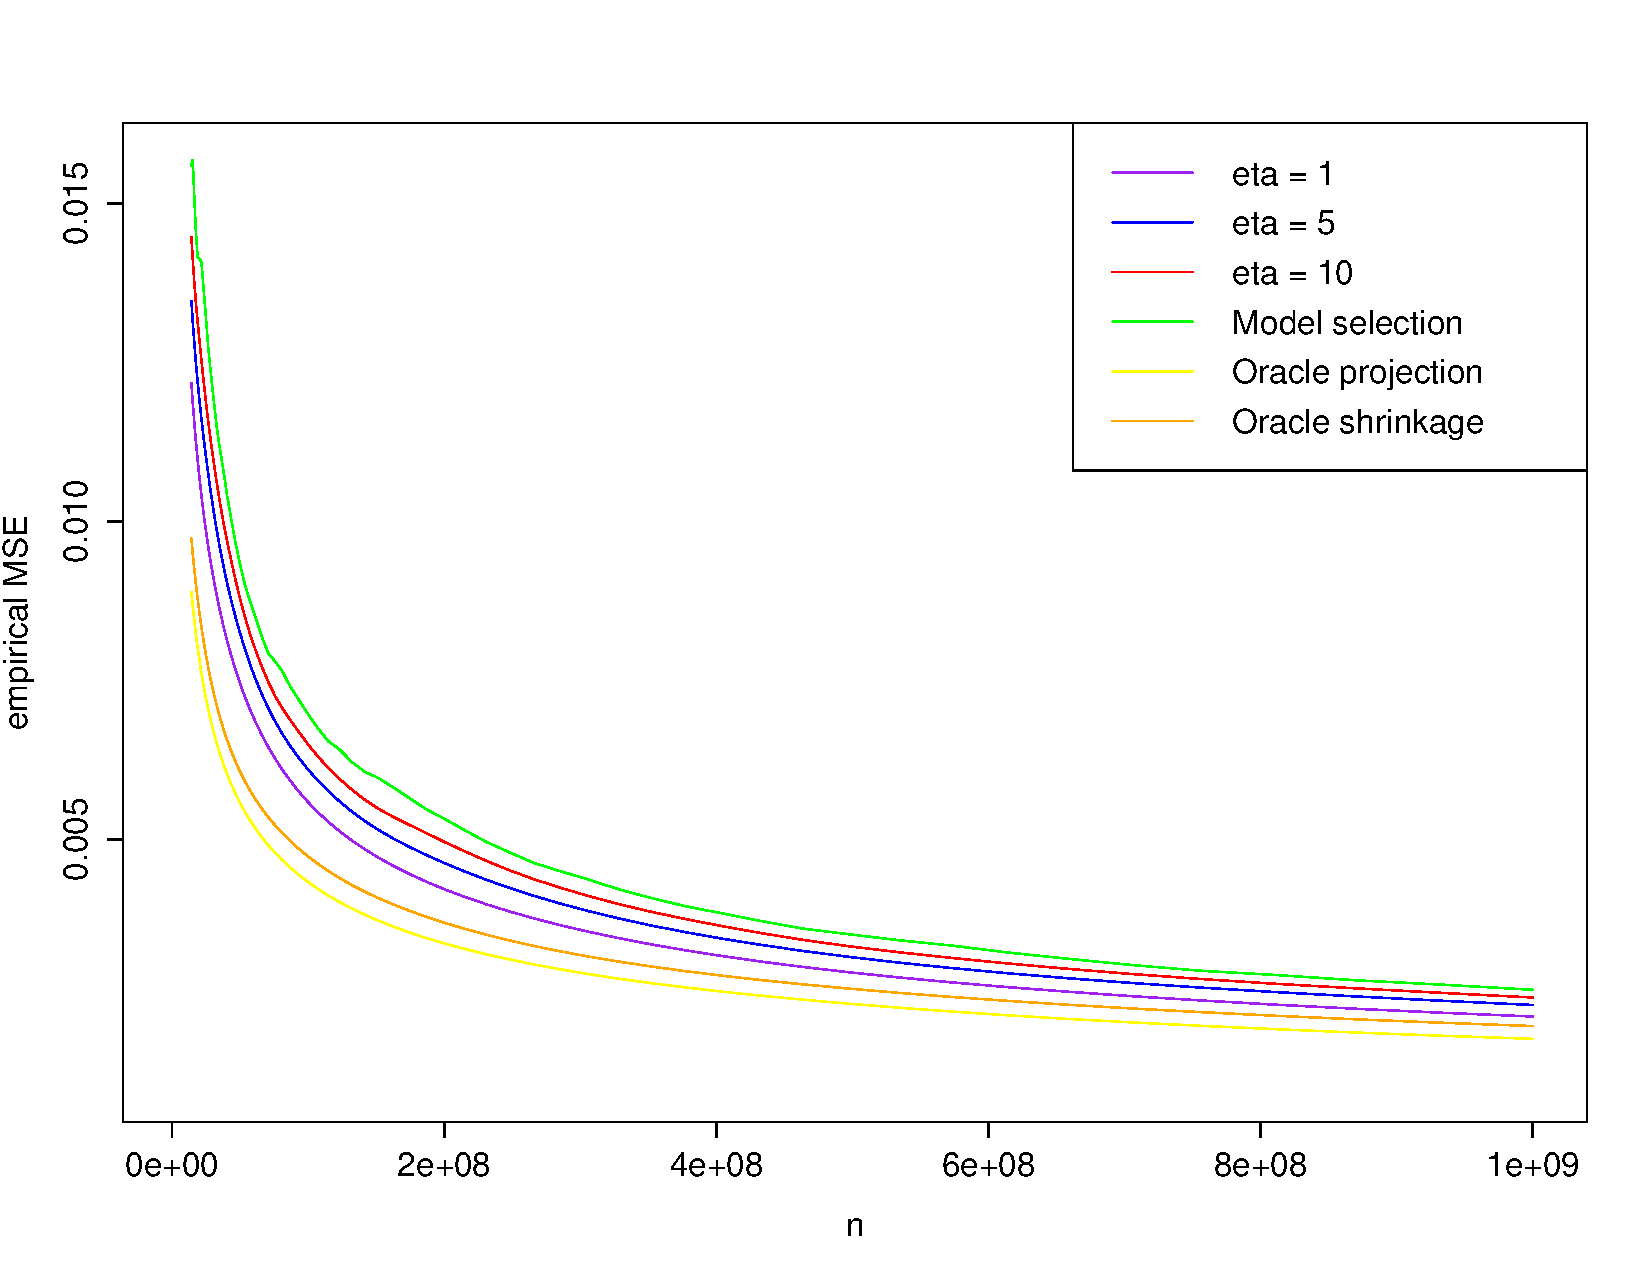
\includegraphics[width=.5\linewidth]{EQM1.pdf}
\caption{Estimated mean of the quadratic error of the Bayes estimate for $\theta^{\circ}$ polynomial.}
\label{EQM}
\end{figure}


\end{block}

%----------------------------------------------------------------------------------------
%	BIBLIOGRAPHY
%----------------------------------------------------------------------------------------
\setbeamercolor{block title}{fg=white,bg=black}
\begin{block}{\rule{0pt}{2.5ex} Bibliography}
\bibliography{biblio}{}
\end{block}

%----------------------------------------------------------------------------------------
%	CONTACT INFORMATION
%----------------------------------------------------------------------------------------

%\setbeamercolor{block title}{fg=black,bg=red!90!black} % Change the block title color
%
%\begin{block}{Contact Information}
%
%\begin{itemize}
%%\item Web: \href{http://www.university.edu/smithlab}{http://www.university.edu/smithlab}
%\item Email: \href{mailto:loizeau@math.uni-heidelberg.de}{loizeau@math.uni-heidelberg.de}
%\item Phone: +49 622 15414186
%\end{itemize}
%
%\end{block}

%----------------------------------------------------------------------------------------

\end{column} % End of the second column

\begin{column}{.02\textwidth}\end{column} % Empty spacer column

\end{columns} % End of all the columns in the poster

\end{frame} % End of the enclosing frame


\bibliographystyle{plainnat}

\end{document}